\section{Wavelet--conditioning: detector for intermittencies}

\subsection{Forced Structures and Natural Structures}%%Lior-This doesn't have to be a subsubsection but should be addressed in this section
As the forced large scale turbulent structures propogate downstream, they produce a nearfield pressure wave signature that has been shown in figure \ref{fig:phaseaxialbothM} for three different excitations, $S_t \in \{ 0.05, 0.15, 0.25 \}$ in the phase-averaged sense. 

It is not possible to use phase--averaging with the unforced case since the structures, although dominated by Strouhal numbers related to the instabilities in the jet, experience enough variation that they can not be captured using phase-averaging at a specific frequency. 
It is necessary to use an alternative averaging method in order to appreciate a similar signature due to unforced jet turbulent--structures.
Instead of phase-averaging, a wavelet--based method, namely wavelet--conditioning, was applied to the unforced and forced cases to determine how closely the forced structures relate to the natural structures in the jet for both the experiments and simulations.

\subsubsection{Wavelet Conditioning Process}
The wavelet--conditioning was used for structure identification in jets and other turbulent flows \cite{Camussi1997,Camussi1997b,Guj1999,Camussi2002,Guj2003}.
The technique is based on the use of the so--called Local Intermittency Measure or LIM, introduced in 1992 by Farge \etal \cite{Farge1992}.
The LIM is the ratio between two energies: a local energy for a specific time and scale $(\tau, s)$ and an averaged energy in time for the same scale $s$.
The LIM was demonstrated to be a well suited indicator for coherent structure identification \cite{Camussi1997}. Its mathematical expression is:
\begin{equation}
	\label{eqn:LIM}
	L(s, \tau) = \frac{w^{2}(s, \tau)}{\left<w^{2}(s, \tau)\right>_{\tau}}
\end{equation}
where $w^{2}(s, \tau)$ is the local energy for a specific time and scale, and $\left< \bullet \right>_{\tau}$ represents a time average.
As a ratio between positive quantities, LIM can only be positive ($L \geqslant 0 $). LIM gives an information about the fluctuation of energy and by choosing a proper threshold $T$ it is possible to select a set of times $\{\tau_{i}\}$ corresponding to peaks with value greater than the threshold $T$.
The peaks are local maxima of LIM and are constrained by the following conditions:
\begin{equation} \label{eqn:thresholdLIM}
    \begin{cases}
        &L(s, \tau) > T,\\
        \\
        &\frac{\partial L}{\partial \tau}(s, \tau) = 0,\\
        \\
        &\frac{\partial^{2} L}{\partial \tau^{2}}(s, \tau) < 0,
    \end{cases}
\end{equation}

% The present work deals with forced and unforced jet. The forced cases are more organized than the unforced and so selecting one threshold for all the different cases is not obvious. The first objective of the use of the wavelet--conditioning in the present work is to validate that experiment and numerical simulation present a similar near--field pressure fluctuations by comparing the signatures of the large scale turbulent--structures. The analysis using the wavelet--conditioning is not time consuming and so instead of selecting one threshold for each case, the analysis was carried out on an ensemble of threshold and the results were selected from the set with the lowest level of noise. Though, different threshold were used for the numercal and experimental database. The threshold value for the numerical database is of 2 while its value is of 5 for the experimental database.

An iterative process was used in order to fix the threshold $T$. To initiate the iterative process it is needed first to select a 'first estimate' of the threshold. It was taken to be equal to 1. The algorithm of the iterative process is applied to each scale of the wavelet--decomposition and allows to have a threshold for each scale. The algorithm used to obtain this is:
\begin{enumerate}
  \item Select a first threshold to initiate the iterative process (1 in the present case)
  \item Evaluate the coefficient
  \begin{equation}
    R(T) = -\frac{\log\left(\frac{N_p}{N_m}\right)}{\log\left(\frac{\sigma_{w_p}}{\sigma_{w_m}}\right)}
  \end{equation}
  where $N_p$ is the length of the set $\{L > T\}$, $N_m$ is the length of the set $\{L \leqslant T\}$, $\sigma_{w_p}$ the standard deviation of the set $\{w\left( \tau_p\right) | L\left( \tau_p \right) > T\}$ and $\sigma_{w_m}$ the standard deviation of the set $\{w\left( \tau_m\right) | L\left( \tau_m \right) \leqslant T\}$
  \item Re-evaluate $T$
  \item Iterate points 2 and 3 until $T$ achieve the maximum of $L$ for the scale under analysis
\end{enumerate}
The outcome of this iterative process is a set of vectors: one containing the different value of $T$ and the second the different value of $R(T)$. The threshold for the analysis is selected to correspond to the maximum of $R(T)$.

The next step is to get similar results to those obtained with the phase--average. In order to get the signatures, a conditional--average (eqn. \ref{eqn:ensembleAverage}) using the set of times $\{\tau_{i}\}$ is performed. In one way, the conditional--average and phase--average are similar: the set of times $\{\tau_{i}\}$ replaces the phases on which the phase--average is performed. At each time location corresponding to a peak of energy, a window $W$ of fixed time--length $l_{W}$ is selected from the original signal $p \left( t \right)$. The conditional--average, $\tilde{p}$ is calculated from this set of windows:
\begin{equation} \label{eqn:ensembleAverage}
    \tilde{p}^n_{m}\left( W \right) = \left< p_{m} | P_{k} \right>_{\tilde{\tau}^n_{s}} = \frac{1}{N^n} \sum^{N^n}_{i = 1} p_{m}\left(\xi_{i}\right),
\end{equation}
where the superscript $n$ and subscript $m$ stand for the position of the reference signal and of any other signal of the array, respectively. Also, the subscript $s$ stands for the scale, $N^n$ is the number of detected events, $\tilde{\tau}^n_{s}$ is the set of corresponding times for a specific scale $s$ at which these events are occurring and $\{\xi_{i}\}$ is the interval surrounding each peak, $\xi_{i} \in \left[ \tilde{t}_{i} - \frac{l_W}{2}, \tilde{t}_{i} + \frac{l_w}{2} \right]$, $\tilde{t}_{i} \in \tilde{\tau}^n_{s}$.
A first analysis using equation \ref{eqn:ensembleAverage} was performed on the microphones line--array. A second analysis was then performed by doing the conditional--average only with peaks with negative/positive value in the real domain (pressure).
\begin{figure}
\centering{}
\subfloat[only negative peaks]{\includegraphics[width=3.2in]{figures/eps/negativePeak.eps}}
\subfloat[only positive peaks]{\includegraphics[width=3.2in]{figures/eps/positivePeak.eps}}

\subfloat[comparison between the signatures]{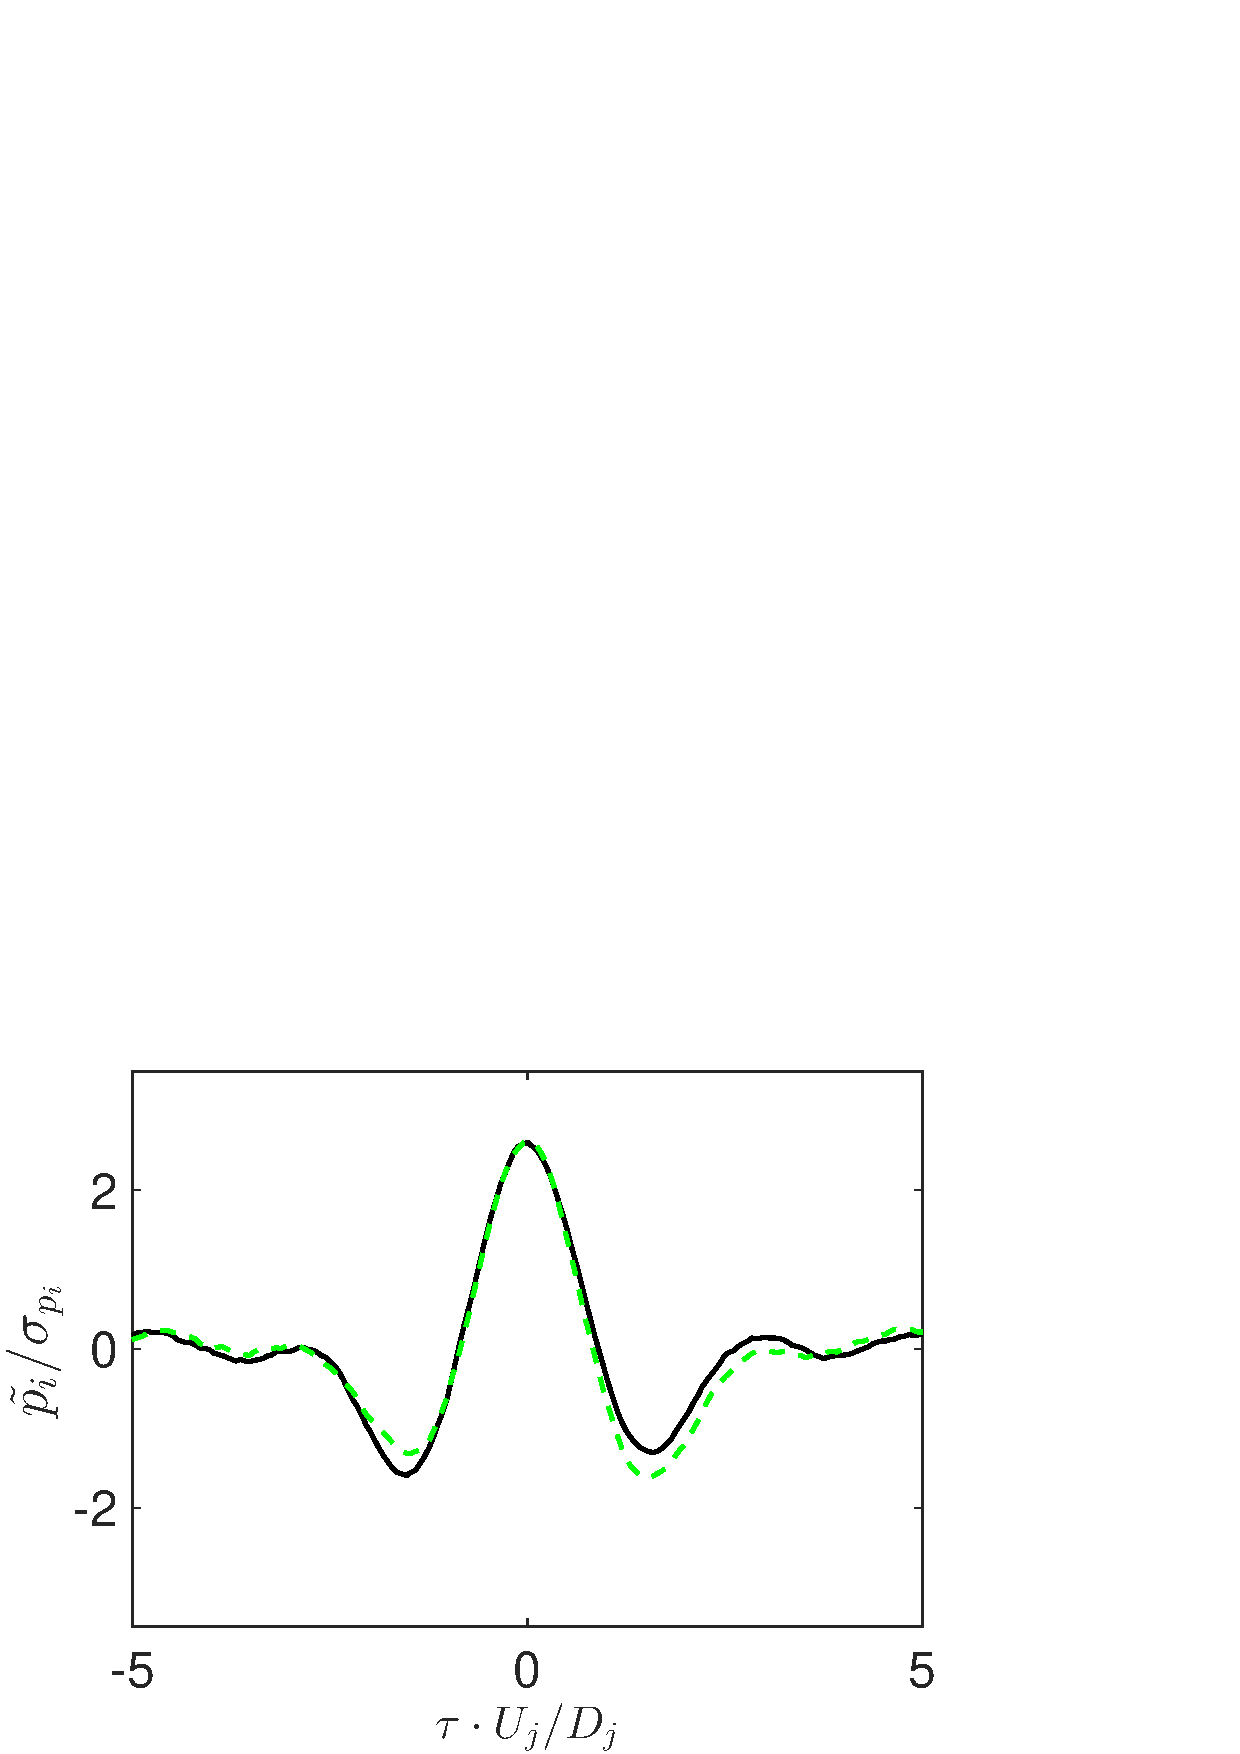
\includegraphics[width=3.2in]{figures/eps/compPeaks}}
\caption{Auto--conditioning signatures of the signal at $x/D = 3$} \label{fig:compPeaks}
\end{figure}
Figure \ref{fig:compPeaks} presents the two subfigures for the different cases (negative/positive peaks) and a third subfigure to compare them.
%\begin{itemize}
%  \item $(a)$ conditional--average (eqn. \ref{eqn:ensembleAverage}) using only the negative peaks
%  \item $(b)$ only the positive peaks
%  \item a comparison between the two previous one ($(a)$ was inverted in order to compare it to $(b)$)
%\end{itemize}
Figure \ref{fig:compPeaks}$(c)$ presents the resemblance between the signature of subfigures $(a)$ and $(b)$ on which the conditional--average was performed using only negative or positive peaks (it is important to understand that the differentiation is done by evaluating the value of each peak in the real domain and not in the LIM/wavelet domain). At this point, it is believed to be the result of the passage of two sucessive large scale turbulent--structures, in the zone where their interaction take place.
% Do you think I should put a scheme here to explain it?
The formulation of the conditional--average was modified to take this observation into account and reformulated as follows:
\begin{equation} \label{eqn:condAvgSign}
  \tilde{p}_{m}^n\left( W \right) = \left< p_{m} | P_{k} \right>_{\tilde{\tau}^n_{s}} = \frac{1}{N^n} \sum^{N^n}_{i = 1} sign\left( p_{n} \left( \tilde{t}_{i} \right) \right) p_{m} \left( \xi_{i} \right),
\end{equation}
$sign\left( p_{n} \left( \tilde{t}_{i} \right) \right)$ is introduced to take into account the sign of the peak in the real domain. This operation might be unnecessary for an experimental database (with a long time--series) but for a numerical database which is strongly limited in its time duration it improves the results obtained with the wavelet--conditioning.
The conditional--average using eqn. \ref{eqn:ensembleAverage} with all the peaks present (not presented here) is not relevant as additional proof for the separation between negative/positive peaks.
When the conditional--average is performed on a signal $p_{n}$ by using its own set of times ${\tilde{\tau}^n_{s}}$, making $n = m$; it becomes the auto--conditioning. If the conditional--average of a signal $p_{m}$ is done by using the set of times of a signal $p_{n}$, and so $n \neq m$; it is then called the cross--conditioning. The auto/cross--conditioning are presented in Fig.  \ref{fig:condNcond}: the top is the auto--conditioning where the selection of $W$ is done in the reference signal $n$; and the bottom is the cross--conditioning of another signal $m$ where $W$ is centered around the times obtained with signal $n$. For more information about the wavelet--transform, see \cite{Farge1992}.
 \begin{figure}[!ht]
\centering
    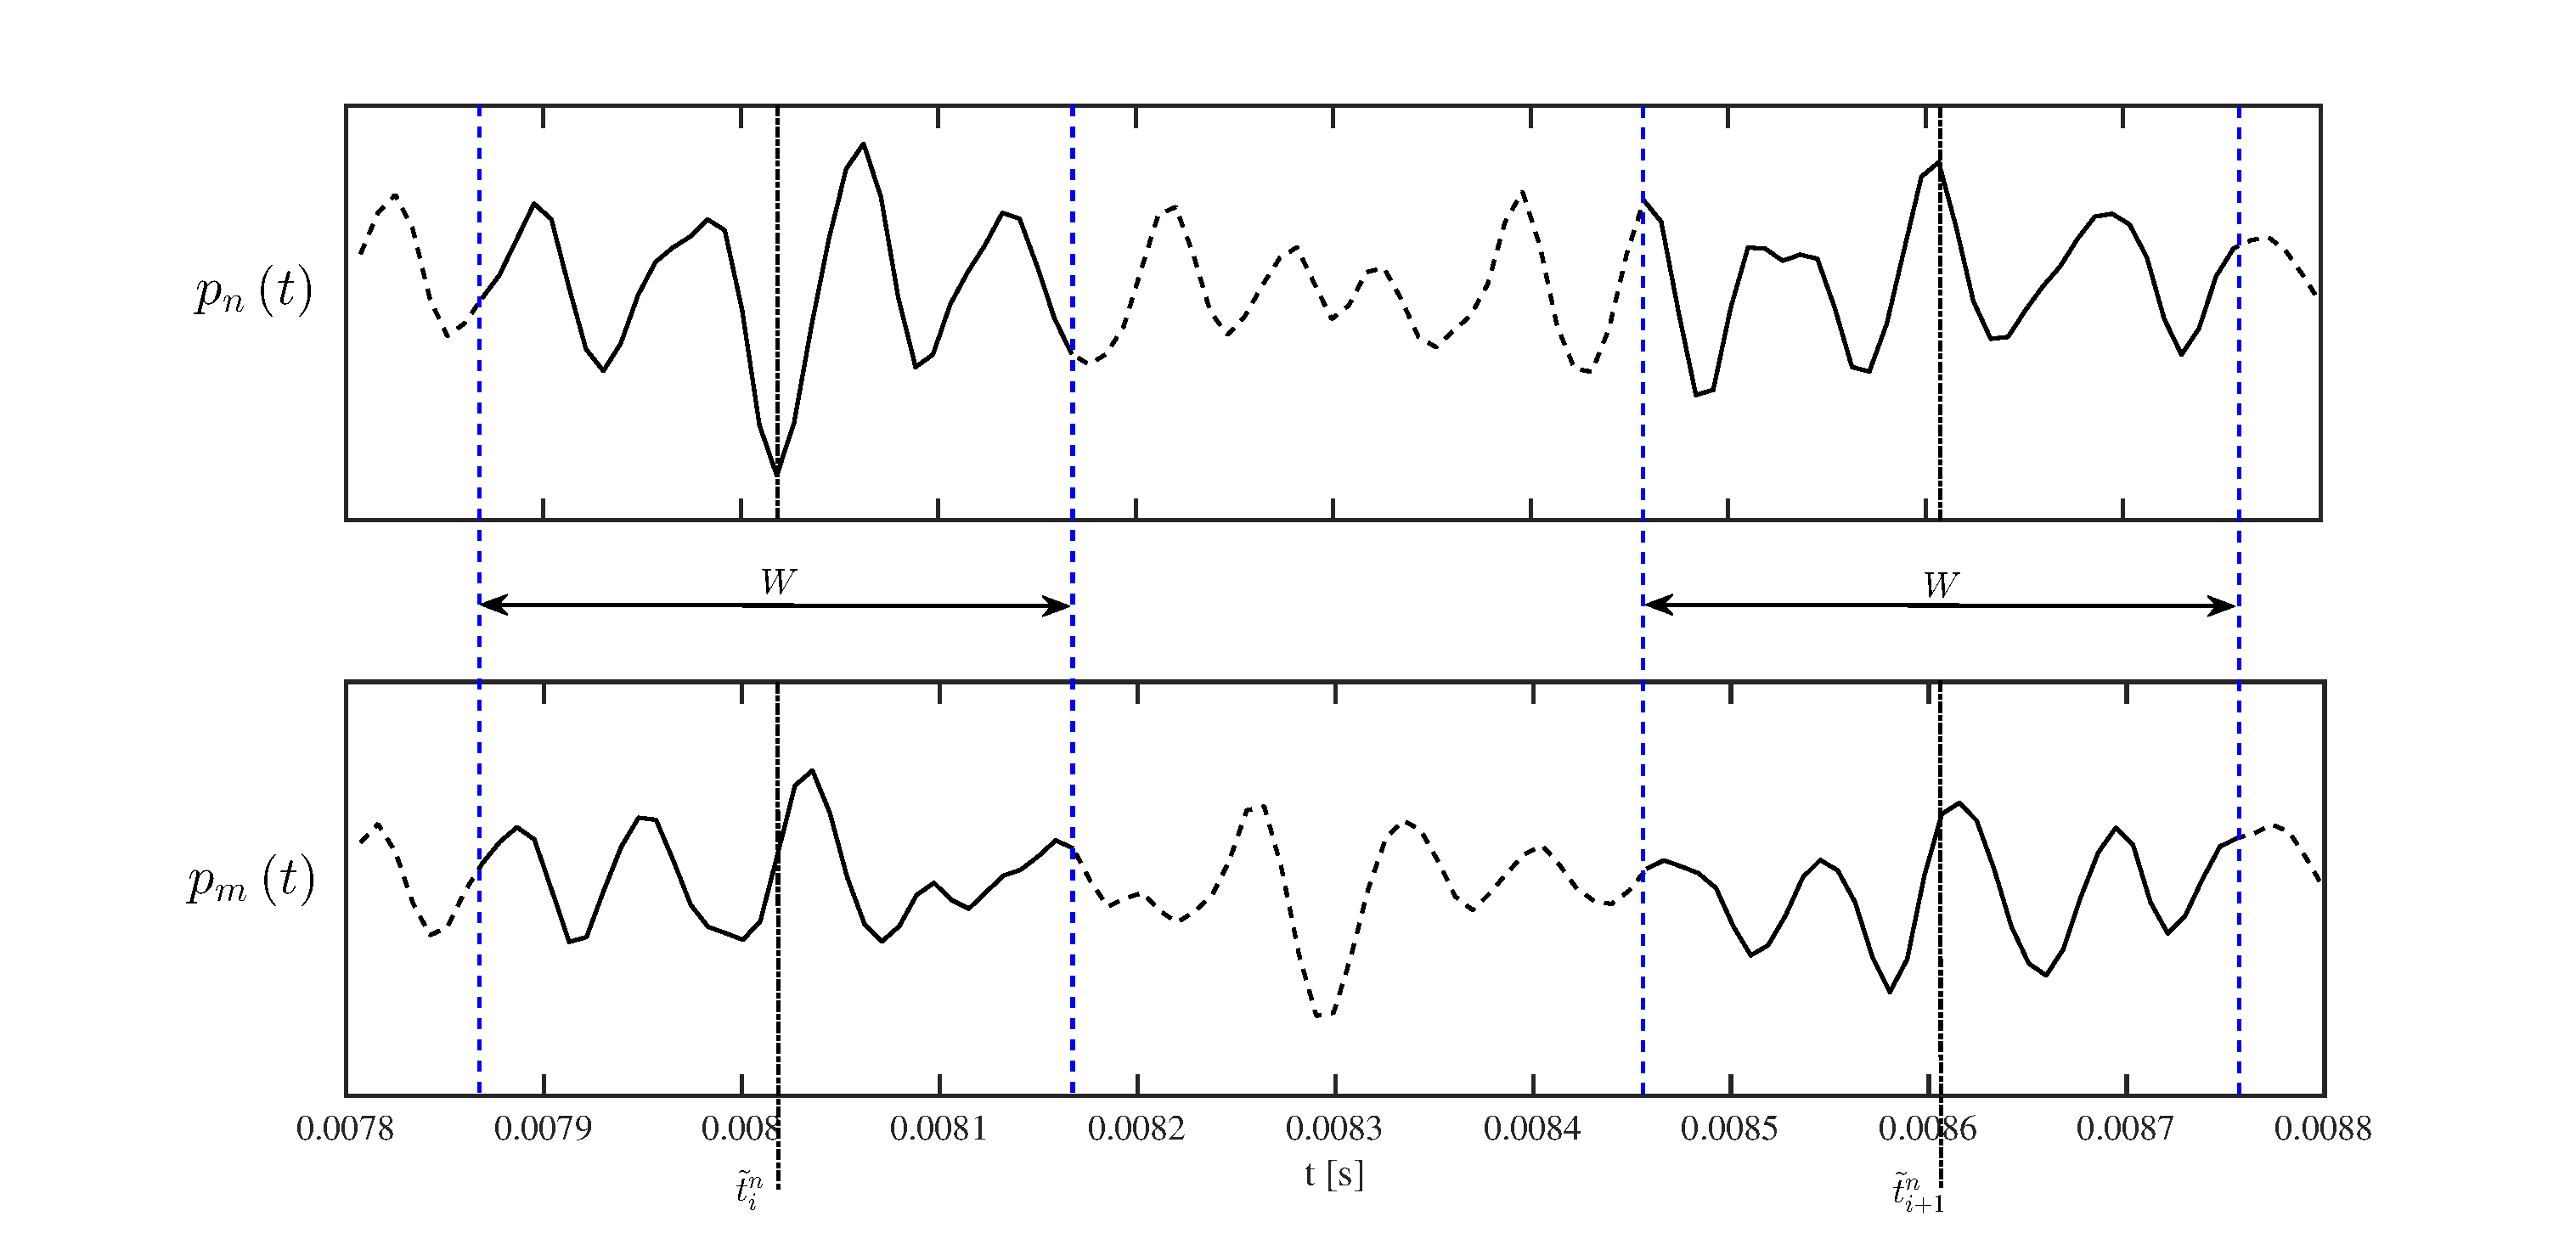
\includegraphics[width=1\textwidth]{figures/pdf/condNcond}
\caption{\textit{Auto--conditioning of a signal $p_n(t)$ and cross--conditioning of a signal $p_n(t)$}}
\label{fig:condNcond}
\end{figure}